\chapter{Introduction}
%------------------
%------------------
\section{Distance running}
    \subsection{Types and competitions}
In competition, \textit{distance running} is split between middle-distance (\SI{800}{m} to \SI{3000}{m}), and long-distance (\SI{3000}{m} and above). A typical competition occurs on a \SI{400}{m} oval running track, or on a closed and measured road course. Athletes aim to either complete the course in as little time as possible, or to obtain the highest possible finishing rank in the field. Either way, an athlete's goal is to run as fast as possible.

Physiologically, performance in competition depends on the athlete's aerobic and anaerobic energy systems, as well as running economy\cite[1]{brandon1995physiological}. An athlete's \votmax and lactate threshold\footnote{The maximal intensity an athlete can sustain without significant accumulation of lactic acid.} are key metrics of fitness in long- and middle-distance running.\cite[9]{brandon1995physiological}. Of course, the relative weight of each factor on performance depends on the race distance: a longer distance relies much more heavily on the aerobic system.
%------------------
%    \subsection{Key factors affecting performance}
%------------------
    \subsection{Differences between elite and recreational runners}
There is no globally accepted definition of what constitutes an elite athlete, or elite distance runner. For the purposes of this article, we define an elite athlete as one who competes at the provincial, national, or international level. At this level of competition, athletes would undergo rigorous training almost every day of the week, year-round. As a result, we would expect to see highly developed physical adaptations as a result of their training protocol. 

On the other end, while a recreational runner can still be competitive\footnote{The vast majority of running competitions are open, such as marathons and road races.}, a recreational runner would not have accumulated sufficient training volume to develop physical adaptations to the extend that an elite athlete would. 

In particular, elite runner have a significantly higher capacity to consume oxygen during aerobic exercise (\vot), as well as efficient running biomechanics which enable them to require less oxygen consumption for a given effort and pace\cite{daniels2013daniels}. These performance metrics will be discussed in more detail in Chapter \ref{ch:performancemetrics}.
%------------------
%------------------
\section{History and popularity of beetroot juice}
    \subsection{Initial research}
Research interest into beetroot juice and exercise science exploded in 2009 following the publication of a University of Exeter study titled \textit{Dietary nitrate supplementation reduces the $O_2$ cost of low-intensity exercise and enhances tolerance to high-intensity exercise in humans}. The study analyzed plasma nitrite concentration, blood pressure, oxygen consumption, and time to exhaustion
in eight male subjects over a 6 day period, as assessed through a step test\footnote{Step tests are a classic estimator of aerobic fitness in which subjects are asked to step on and off a shallow raised platform.\cite{brouha1943step}}.
The results suggested that beetroot juice, due to its high concentration of inorganic nitrate, reduced systolic blood pressure and oxygen consumption, and increased time to exhaustion\cite{bailey2009dietary}.

%------------------
    \subsection{Running and popular culture}
    \begin{figure}
        \centering
        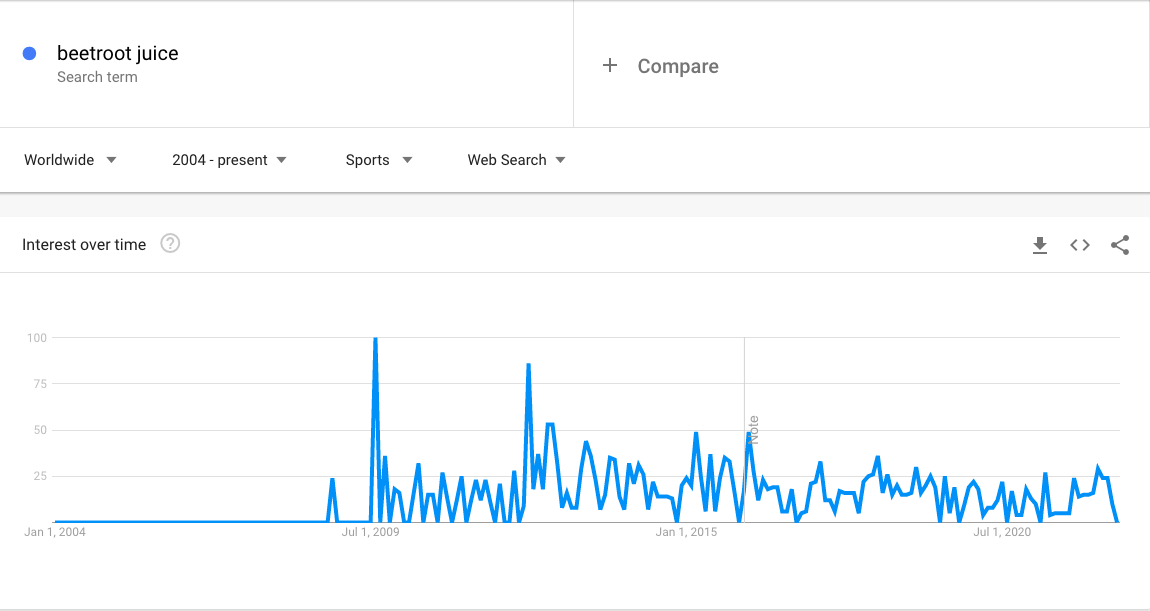
\includegraphics[width=1.0\textwidth]{assets/googletrends.png}
        \caption{Worldwide Google Trend for the query \texttt{beet juice} in the \texttt{Sports} category. The first spike in 2009 results from the Bailey study at the University of Exeter, followed by a number of popular media articles.}
        \label{fig:googletrends}
    \end{figure}
Following the publication of the University of Exeter article, various popular science media outlets (for example, Science Daily\cite{sciencedaily_2009}) reported on the benefits of beetroot juice.  In November of 2009, \textit{Runner's World Magazine} writer Amby Burfoot published an article called \textit{Why Blood Dope When Drinking Blood-Red Beet Juice Is Just About As Good?}\cite{burfoot_2020} The hype took off, and the beverage became a staple for runners, both elite and recreational, in their preparation for competition.
%------------------
    \subsection{Commercial products}
The rising interest in beetroot juice within the running community spawned a number of commercial products claiming to deliver these performance benefits to athletes. In the UK, a company called Beet It\textregistered advertises sets of 15 bottles of single-serving beetroot juice concentrate containing \SI{400}{mg} of nitrates. At time of writing, the case is sold for CAD\$62.99 through their Canadian online retail portal. Similar products targeted specifically to athletes are available in the US, UK, and Europe; however Beet It\textregistered appears to be the only product on the market which declares the nitrate content on the label. Of course, common beet juice is also available in many grocery stores, although these products are not specifically marketed for their benefits to athletic performance. That being said, it begs the question: are these supplements effective and if so, to whom, and to what extent?
\begin{figure}
    \centering
    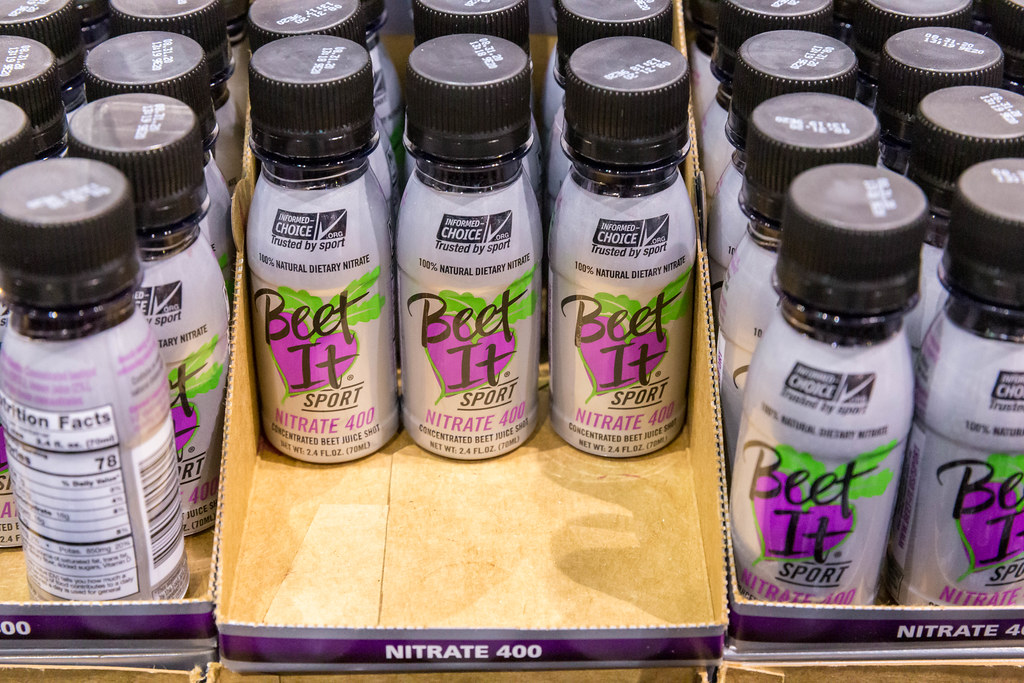
\includegraphics[width=0.65\textwidth]{assets/beetit.jpg}
    \caption{Beet It\textregistered{} bottles of commercially available nitrate-rich beetroot juice concentrate. (\textcopyright{} Marco Verch, 2019, \url{https://www.flickr.com/photos/160866001@N07/48881775563}. Obtained under Creative Commons \href{https://creativecommons.org/licenses/by/4.0/legalcode}{Attribution 4.0 International Public License})}
    \label{fig:beetit}
\end{figure}